\documentclass[xetex,mathserif,serif,aspectratio=169]{beamer}

\usepackage{xltxtra}
\usepackage{color}
\usepackage{url}
\usepackage{listings}
\usepackage{fontspec}
\usepackage{geometry}
\usepackage{lastpage}
\usepackage{fancyhdr}
\usepackage{amsmath}
\usepackage{amsthm}
\usepackage{amssymb}
\usepackage{blkarray}
\usepackage{multicol}
\usepackage{relsize}
\usepackage{listings}
\usepackage{xunicode}
\usepackage{xltxtra}
\usepackage{color}
\usepackage{url}
\usefonttheme[onlymath]{serif}

\definecolor{solarized@base03}{HTML}{002B36}
\definecolor{solarized@base02}{HTML}{073642}
\definecolor{solarized@base01}{HTML}{586e75}
\definecolor{solarized@base00}{HTML}{657b83}
\definecolor{solarized@base0}{HTML}{839496}
\definecolor{solarized@base1}{HTML}{93a1a1}
\definecolor{solarized@base2}{HTML}{EEE8D5}
\definecolor{solarized@base3}{HTML}{FDF6E3}
\definecolor{solarized@yellow}{HTML}{B58900}
\definecolor{solarized@orange}{HTML}{CB4B16}
\definecolor{solarized@red}{HTML}{DC322F}
\definecolor{solarized@magenta}{HTML}{D33682}
\definecolor{solarized@violet}{HTML}{6C71C4}
\definecolor{solarized@blue}{HTML}{268BD2}
\definecolor{solarized@cyan}{HTML}{2AA198}
\definecolor{solarized@green}{HTML}{859900}
\definecolor{yaleblue}{HTML}{0E4C92}

\newcommand{\yellow}[1]{\textcolor{solarized@yellow}{#1}}
\newcommand{\orange}[1]{\textcolor{solarized@orange}{#1}}
\newcommand{\red}[1]{\textcolor{solarized@red}{#1}}
\newcommand{\magenta}[1]{\textcolor{solarized@magenta}{#1}}
\newcommand{\violet}[1]{\textcolor{solarized@violet}{#1}}
\newcommand{\blue}[1]{\textcolor{solarized@blue}{#1}}
\newcommand{\cyan}[1]{\textcolor{solarized@cyan}{#1}}
\newcommand{\green}[1]{\textcolor{solarized@green}{#1}}
\newcommand{\yblue}[1]{\textcolor{yaleblue}{#1}}
\newcommand{\base}[1]{\textcolor{solarized@base01}{#1}}


\defaultfontfeatures{Mapping=tex-text}
\hypersetup{pdfstartview={FitH}}

\newcommand{\old}[1]{\fontspec[Alternate=1,Ligatures={Common}]{Hoefler Text}\fontsize{18pt}{30pt}\selectfont #1}%
\newcommand{\oldA}[1]{\fontspec[Alternate=1,Ligatures={Common, Rare}]{Hoefler Text}\fontsize{12pt}{15pt}\selectfont #1}%
\newcommand{\oldB}[1]{\fontspec[Ligatures={Common}]{Didot}\fontsize{12pt}{15pt}\color{solarized@base02}\selectfont #1}%
\newcommand{\tfont}[1]{\fontspec[Alternate=1,Ligatures={Common}]{Hoefler Text}\fontsize{12pt}{20pt}\selectfont #1}%
\newcommand{\dfont}[1]{\fontspec[Ligatures={Common}]{Didot}\fontsize{12pt}{12pt}\selectfont #1}%

\setbeamerfont{title}{family=\old}
\setbeamerfont{author}{family=\tfont}%
\setbeamerfont{frametitle}{family=\oldA}
\setbeamerfont{date}{family=\dfont}

\setbeamertemplate{navigation symbols}{}
\setbeamertemplate{footline}[text line]{%
  \parbox{0.99\linewidth}{
    \normalsize\vspace*{-24pt}\hfill{\color{solarized@base00}\insertframenumber/\inserttotalframenumber}
  }
}


\setlength{\parindent}{0pt}
\setlength{\parskip}{12pt}

\setbeamercolor{structure}{bg=solarized@base3, fg=solarized@base02}
\setbeamercolor{titlelike}{fg=solarized@cyan}
\setbeamercolor{title}{fg=solarized@blue}
\setbeamercolor{subtitle}{fg=solarized@magenta}
\setbeamercolor{alerted text}{fg=orange}
\setbeamercolor{itemize}{fg=solarized@base02}
\setbeamercolor{background canvas}{bg=solarized@base3}
\setbeamercolor{enumerate subitem}{fg=solarized@base02}

\newcommand{\minimize}{\mathop{\mathrm{minimize}}}
\newcommand{\argmin}{\mathop{\mathrm{arg\,min}}}
\newcommand{\argmax}{\mathop{\mathrm{arg\,max}}}
\newcommand{\st}{\mathop{\mathrm{subject\,\,to}}}



\begin{document}

%%%%%%%%%%%%%%%%%%%%%%%%%%%%%%%%%%%%%%%%%%%%%%%%%%%
\begin{frame}[fragile] \frametitle{} \oldB \small

\vfill

{\fontsize{0.7cm}{0cm}\selectfont Lecture 02 \\\vspace{0.2cm} Linear classification methods I}\\\vspace{0.5cm}
22 January 2016

\vspace{2cm}

\begin{minipage}{0.6\textwidth}
Taylor B. Arnold \\
Yale Statistics \\
STAT 365/665
\end{minipage}
\hfill
\begin{minipage}{0.3\textwidth}\raggedleft

\includegraphics[scale=0.3]{../yale-logo.png}
\end{minipage}%

\end{frame}

%%%%%%%%%%%%%%%%%%%%%%%%%%%%%%%%%%%%%%%%%%%%%%%%%%%
\begin{frame}[fragile] \frametitle{} \oldB \small

\textbf{Course website:}

A copy of the whole course syllabus, including a more detailed description
of topics I plan to cover are on the course website.

\begin{center}
\url{http://www.stat.yale.edu/~tba3/stat665/}
\end{center}

This is where all lecture notes, homeworks, and other references will appear.

\pause The first problem set is now posted.

\end{frame}

%%%%%%%%%%%%%%%%%%%%%%%%%%%%%%%%%%%%%%%%%%%%%%%%%%%
\begin{frame}[fragile] \frametitle{} \oldB \small

\textbf{Some thoughts from course survey}

\begin{enumerate}
\item several people mentioned Matlab as alternative
  to R or Python
\item equal interest in CV and NLP
\item requests for finance and biological applications
\item several requests for explaining methods for large,
  distributed computations (Hadoop, Spark, MPI)
\item a diverse set of background in statistics, computer science,
  and data analysis
\end{enumerate}

\end{frame}

%%%%%%%%%%%%%%%%%%%%%%%%%%%%%%%%%%%%%%%%%%%%%%%%%%%
\begin{frame}[fragile] \frametitle{} \oldB \small

Today, we will consider \blue{$1$-dimensional non-parametric regression}.
Specifically, we will consider observing $n$ pairs $(x_i,y_i)$ such
that:
\begin{align*}
y_i &= g(x_i) + \epsilon_i
\end{align*}
For an unknown function $g$ and random variable $\epsilon_i$, where the mean
of the random variable is zero.

\pause You are free to think of the errors being independent, identically
distributed and with finite variances. You may even assume that they are
normally distributed.

\end{frame}

%%%%%%%%%%%%%%%%%%%%%%%%%%%%%%%%%%%%%%%%%%%%%%%%%%%
\begin{frame}[fragile] \frametitle{} \oldB \small

Our goal is to estimate the function $g$. More specifically,
we want to estimate the value of $g$ at the input point $x_{new}$,
denoted as $\widehat{g}(x_{new})$.

\pause The value of $x_{new}$ may be in the original set and it may
not be; however, we assume that $\epsilon_{new}$ is an
entirely different random sample.

\pause Next class I will cover more of the details about training, testing,
validation, and other techniques for evaluating how well a predictive
model is performing. Today we will just spend some time introducing
several standard techniques and gaining some intuition about them.

\end{frame}


%%%%%%%%%%%%%%%%%%%%%%%%%%%%%%%%%%%%%%%%%%%%%%%%%%%
\begin{frame}[fragile] \frametitle{} \oldB \small

The specific methods I will introduce are:

\begin{enumerate}
\item k-nearest neighbors (knn)
\item kernel smoothing (Nadaraya-Watson estimator)
\item linear regression (OLS)
\item local regression (LOESS)
\end{enumerate}

\end{frame}

%%%%%%%%%%%%%%%%%%%%%%%%%%%%%%%%%%%%%%%%%%%%%%%%%%%
\begin{frame}[fragile] \frametitle{} \oldB \small

Here is an example dataset that we will use to illustrate these
four techniques:
\begin{center}
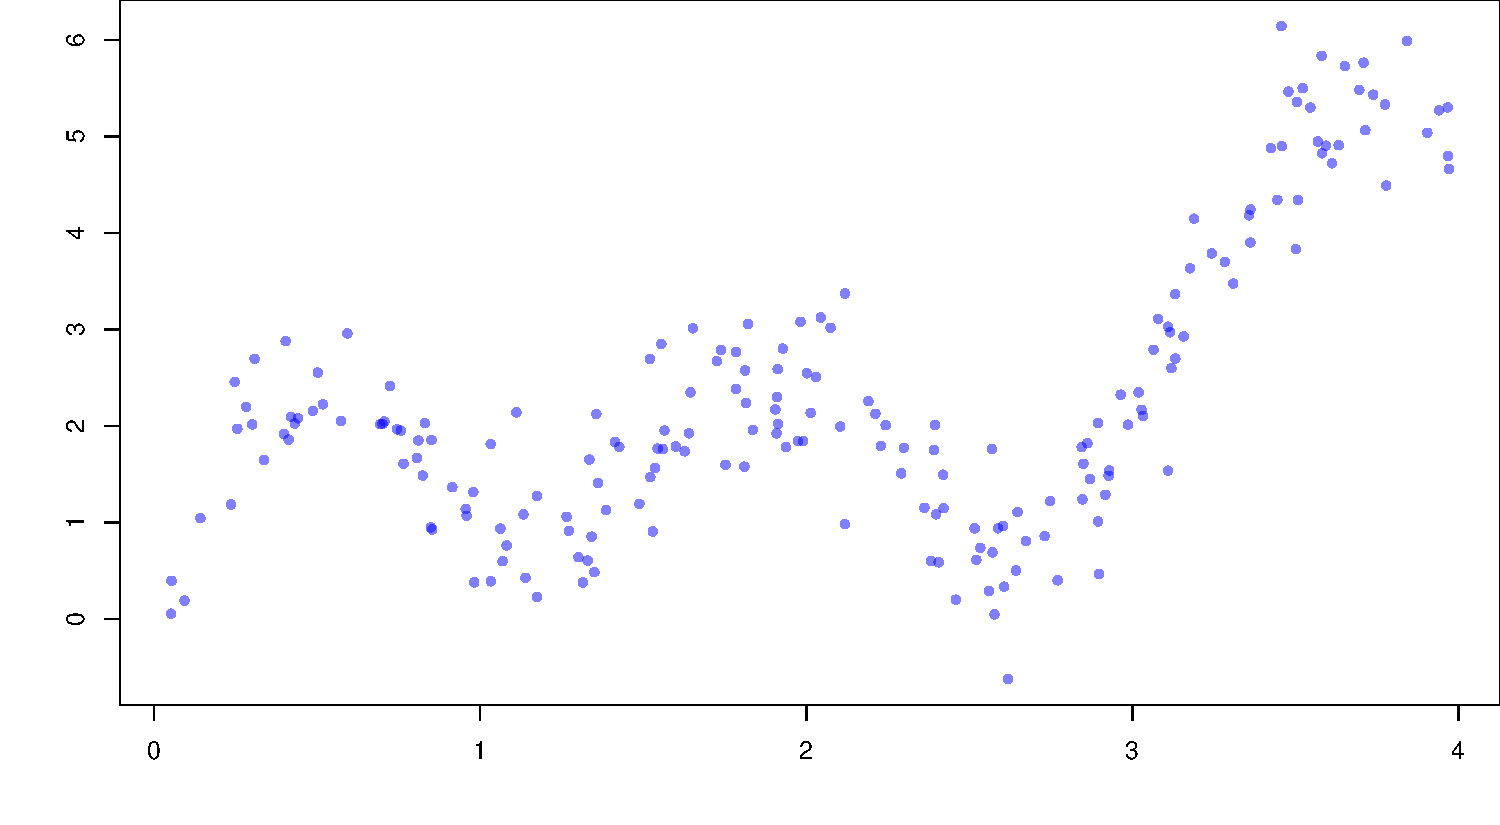
\includegraphics[width=\textwidth]{img/scatter.pdf}
\end{center}

\end{frame}

%%%%%%%%%%%%%%%%%%%%%%%%%%%%%%%%%%%%%%%%%%%%%%%%%%%
\begin{frame}[fragile] \frametitle{} \oldB \small

\yblue{\textbf{k-Nearest neighbors (knn)}}

One of the most straightforward estimators, knn simply sets $\widehat{g}(x_{new})$ to be
the average value of the observed $y$ of the $k$ closest points $x_j$ to $x_{new}$.

\end{frame}

%%%%%%%%%%%%%%%%%%%%%%%%%%%%%%%%%%%%%%%%%%%%%%%%%%%
\begin{frame}[fragile] \frametitle{} \oldB \small

\begin{center}
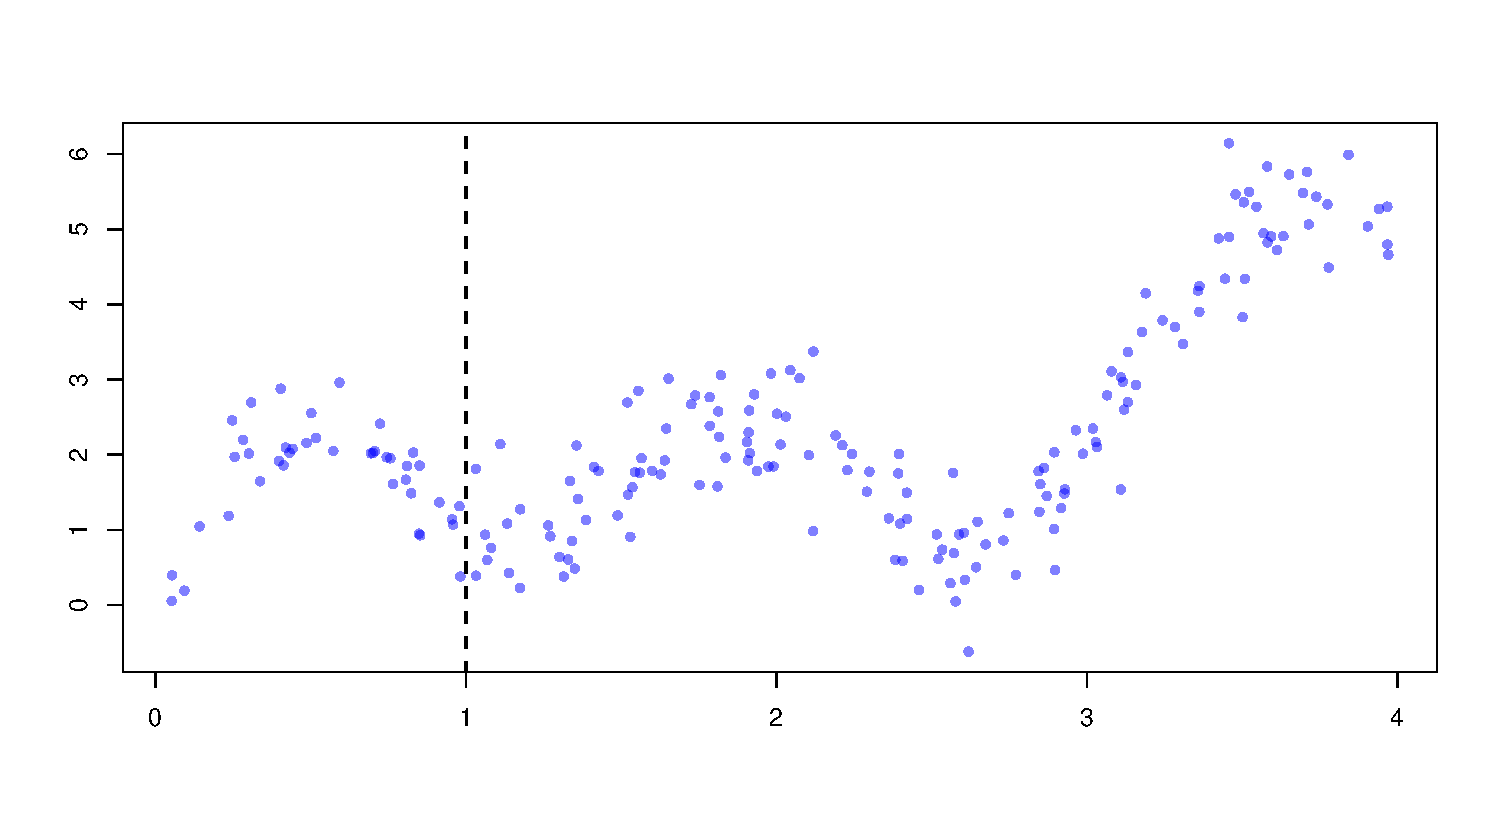
\includegraphics[width=\textwidth]{img/knn1.pdf}
\end{center}

\end{frame}

%%%%%%%%%%%%%%%%%%%%%%%%%%%%%%%%%%%%%%%%%%%%%%%%%%%
\begin{frame}[fragile] \frametitle{} \oldB \small

\begin{center}
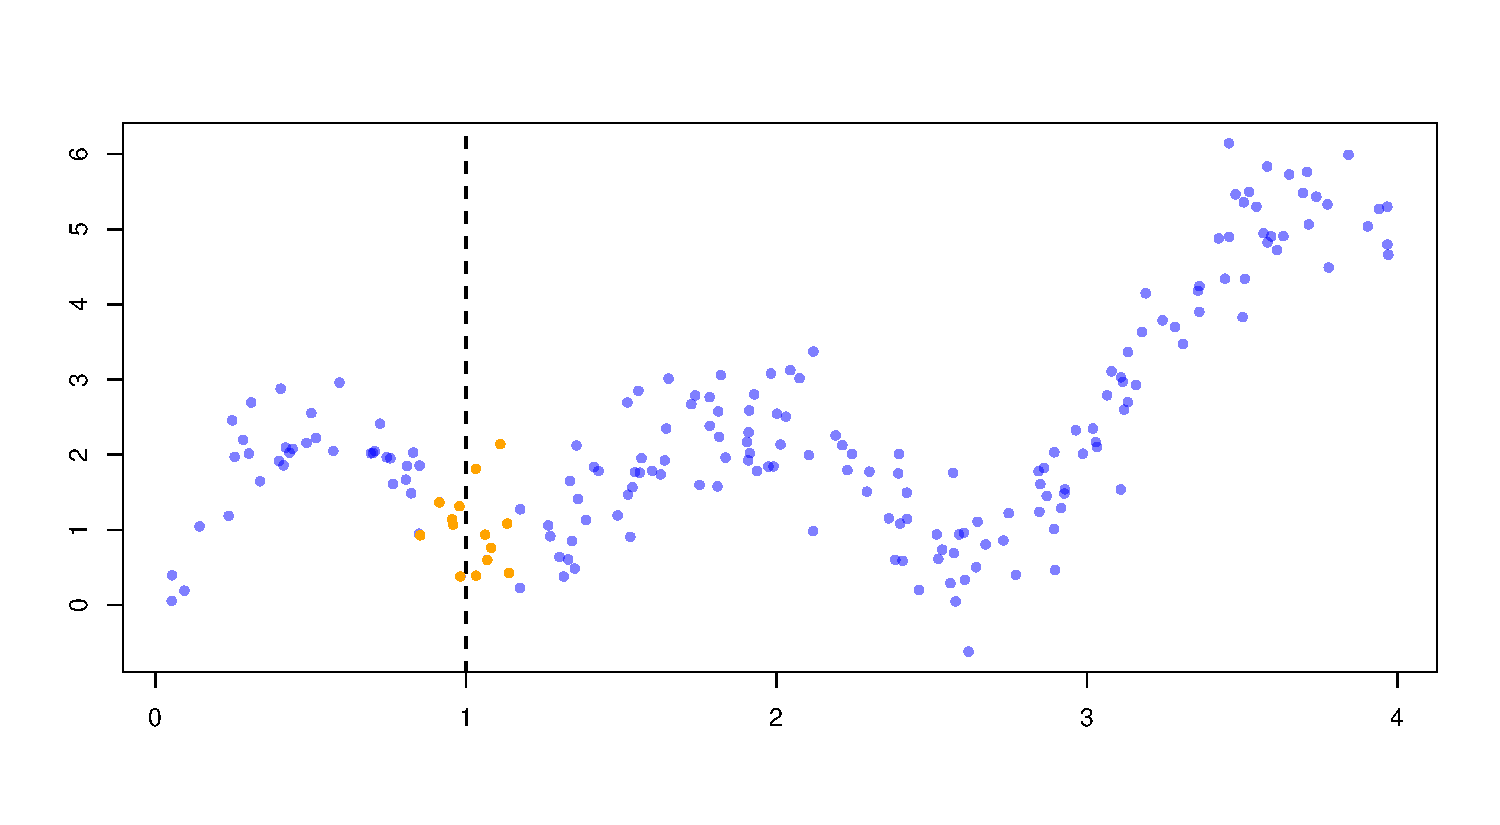
\includegraphics[width=\textwidth]{img/knn2.pdf}
\end{center}

\end{frame}

%%%%%%%%%%%%%%%%%%%%%%%%%%%%%%%%%%%%%%%%%%%%%%%%%%%
\begin{frame}[fragile] \frametitle{} \oldB \small

\begin{center}
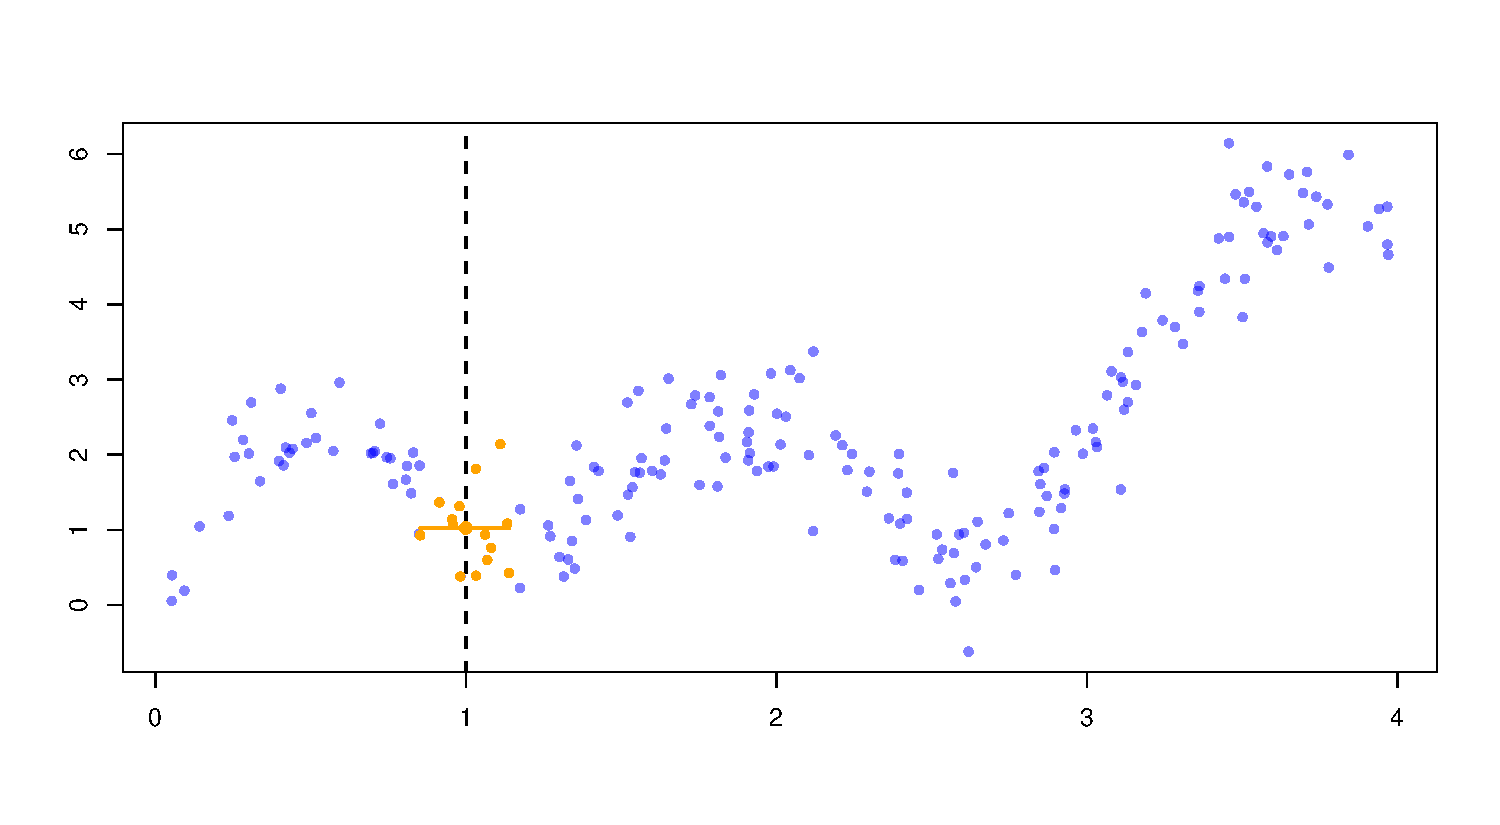
\includegraphics[width=\textwidth]{img/knn3.pdf}
\end{center}

\end{frame}

%%%%%%%%%%%%%%%%%%%%%%%%%%%%%%%%%%%%%%%%%%%%%%%%%%%
\begin{frame}[fragile] \frametitle{} \oldB \small

\begin{center}
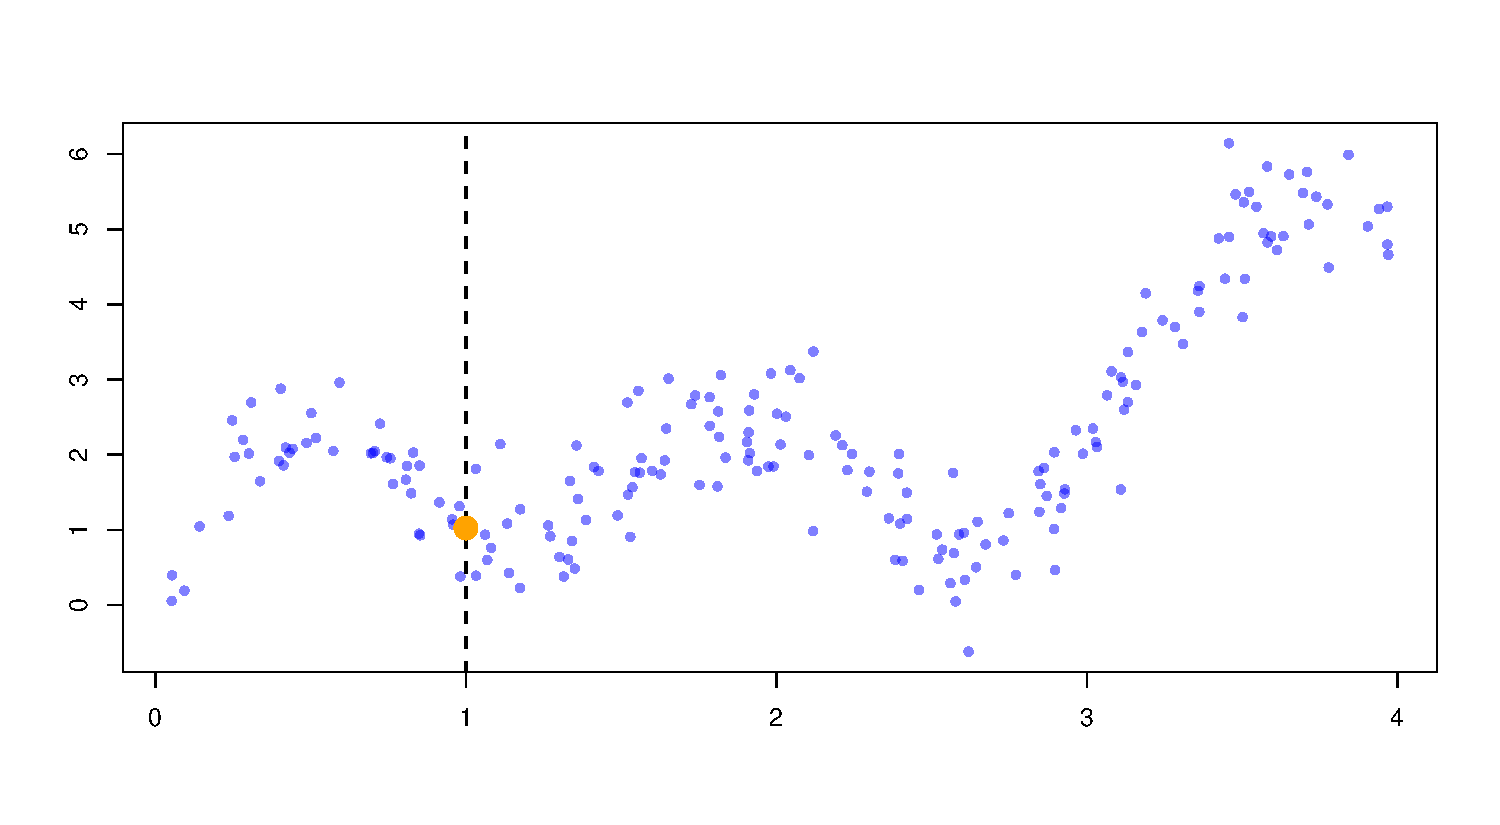
\includegraphics[width=\textwidth]{img/knn4.pdf}
\end{center}

\end{frame}

%%%%%%%%%%%%%%%%%%%%%%%%%%%%%%%%%%%%%%%%%%%%%%%%%%%
\begin{frame}[fragile] \frametitle{} \oldB \small

\yblue{\textbf{k-Nearest neighbors (knn)}}

How might you expect the optimal parameter $k$ to change as $n$ increases?

\end{frame}

%%%%%%%%%%%%%%%%%%%%%%%%%%%%%%%%%%%%%%%%%%%%%%%%%%%
\begin{frame}[fragile] \frametitle{} \oldB \small

\yblue{\textbf{Kernel smoother}}

Rather than averaging the $k$-closest points, kernel smoothers average
observations in the dataset using weights that are inversely proportional
to the distance from the prediction point.

\end{frame}

%%%%%%%%%%%%%%%%%%%%%%%%%%%%%%%%%%%%%%%%%%%%%%%%%%%
\begin{frame}[fragile] \frametitle{} \oldB \small

\yblue{\textbf{Kernel smoothers}}

As an example, consider this estimator
\begin{align*}
\widehat{g}(x_{new}) &= \frac{\sum_i y_i \cdot \phi(||x_i - x_{new}||_2^2) }{\sum_i \phi(||x_i - x_{new}||_2^2)}
\end{align*}
Where $\phi$ is defined as the density function of a standard normal distribution:
\begin{align*}
\phi(z) &= \frac{1}{\sqrt{2\pi}} e^{-z^2/2}
\end{align*}

\end{frame}


%%%%%%%%%%%%%%%%%%%%%%%%%%%%%%%%%%%%%%%%%%%%%%%%%%%
\begin{frame}[fragile] \frametitle{} \oldB \small

\yblue{\textbf{Kernel smoothers}}

The function $\phi$ can be replaced with any other function that you
would like to use. It is often replaced by a truncated variant, as
observations more than a few standard deviations do not give a
noticeable impact on the result.

\end{frame}

%%%%%%%%%%%%%%%%%%%%%%%%%%%%%%%%%%%%%%%%%%%%%%%%%%%
\begin{frame}[fragile] \frametitle{} \oldB \small

\yblue{\textbf{Kernel smoothers - bandwidth}}

What is the main tuning parameter for kernel smoothers? We need to modify
our estimator slightly to include the \blue{bandwidth} parameter $h$:
\begin{align*}
\widehat{g}(x_{new}) &= \frac{\sum_i y_i \cdot \phi(||x_i - x_{new}||_2^2 / h) }{\sum_i \phi(||x_i - x_{new}||_2^2 / h)}
\end{align*}
What does the bandwidth control?

\pause Why might we think of the bandwidth as a standard deviation?

\end{frame}


%%%%%%%%%%%%%%%%%%%%%%%%%%%%%%%%%%%%%%%%%%%%%%%%%%%
\begin{frame}[fragile] \frametitle{} \oldB \small

\begin{center}
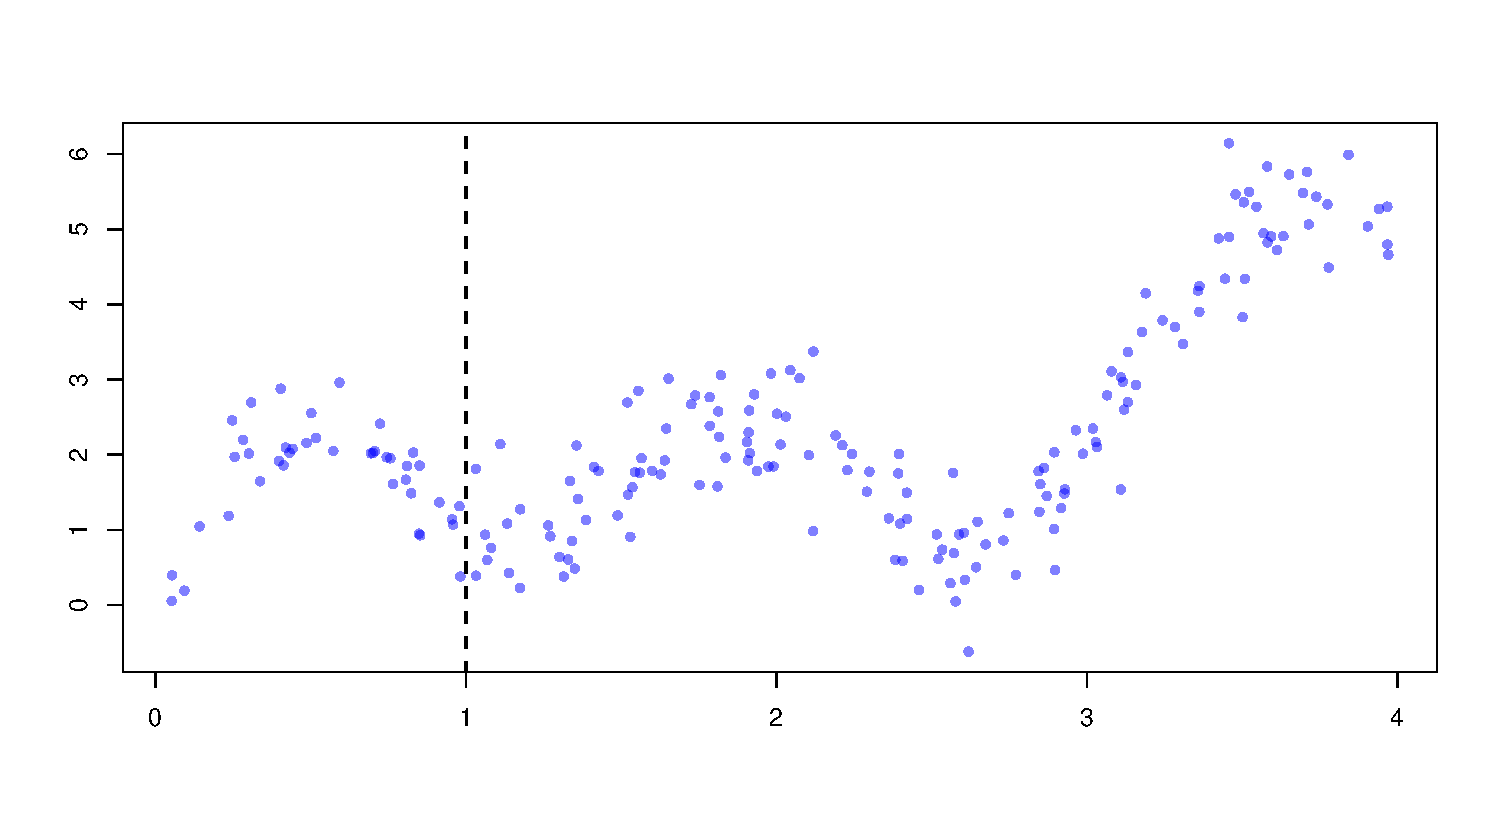
\includegraphics[width=\textwidth]{img/ksmooth1.pdf}
\end{center}

\end{frame}

%%%%%%%%%%%%%%%%%%%%%%%%%%%%%%%%%%%%%%%%%%%%%%%%%%%
\begin{frame}[fragile] \frametitle{} \oldB \small

\begin{center}
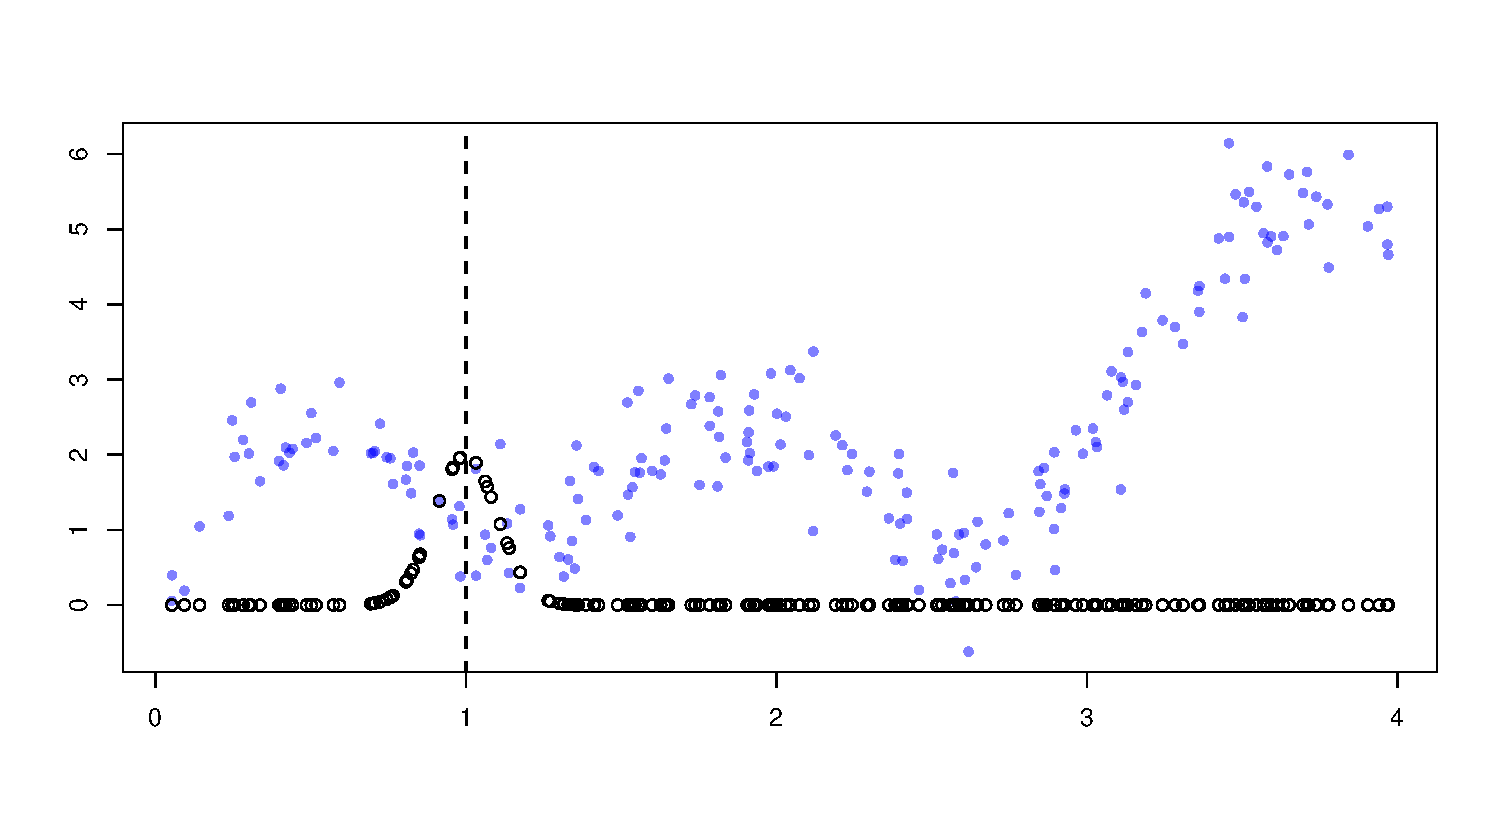
\includegraphics[width=\textwidth]{img/ksmooth2.pdf}
\end{center}

\end{frame}

%%%%%%%%%%%%%%%%%%%%%%%%%%%%%%%%%%%%%%%%%%%%%%%%%%%
\begin{frame}[fragile] \frametitle{} \oldB \small

\begin{center}
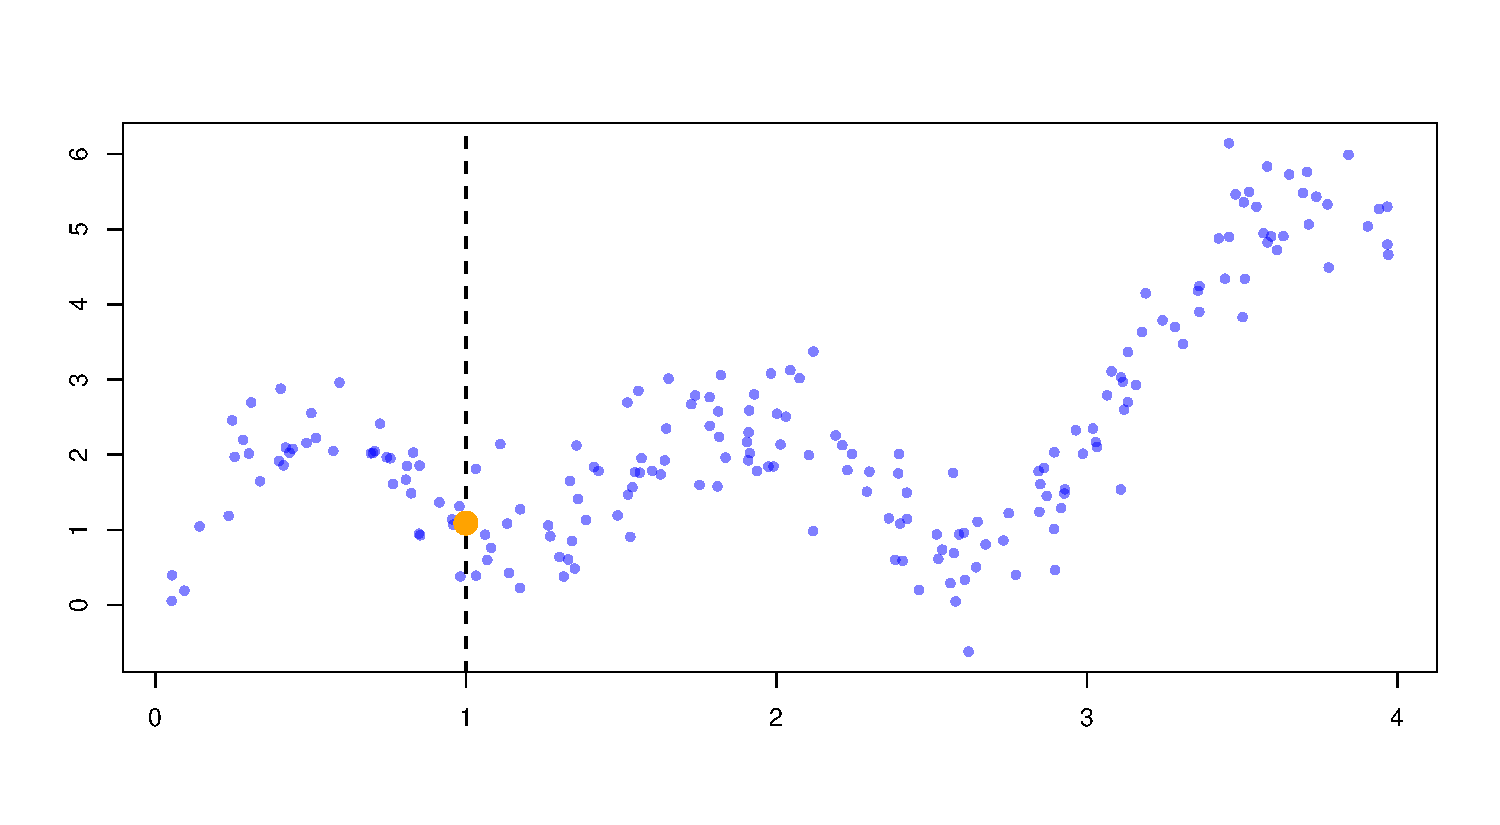
\includegraphics[width=\textwidth]{img/ksmooth3.pdf}
\end{center}

\end{frame}

%%%%%%%%%%%%%%%%%%%%%%%%%%%%%%%%%%%%%%%%%%%%%%%%%%%
\begin{frame}[fragile] \frametitle{} \oldB \small

\yblue{\textbf{Linear regression}}

Hopefully you have already seen linear regression in
some context. Recall that here we assume the data are
generated by a process that looks something like this:
\begin{align*}
y_i &= x_{1,i} \beta_1 + x_{2,i} \beta_2 + \cdots + x_{p,1} \beta_p + \epsilon_i
\end{align*}
For some random variable $\epsilon_i$ and fixed (but unknown)
parameters $\beta_j$.

The parameters $\beta_j$ are most commonly estimated by finding
the values that minimize the squared residuals (known as ols, or ordinary
least squares).

\end{frame}

%%%%%%%%%%%%%%%%%%%%%%%%%%%%%%%%%%%%%%%%%%%%%%%%%%%
\begin{frame}[fragile] \frametitle{} \oldB \small

\yblue{\textbf{Linear regression}}

In our one dimensional case, even including an intercept, this does
not seem very interesting as we have only two parameters to use to
fit the data:
\begin{align*}
y_i &= \beta_0 + x_i \beta_1 + \epsilon_i
\end{align*}

\end{frame}

%%%%%%%%%%%%%%%%%%%%%%%%%%%%%%%%%%%%%%%%%%%%%%%%%%%
\begin{frame}[fragile] \frametitle{} \oldB \small

\begin{center}
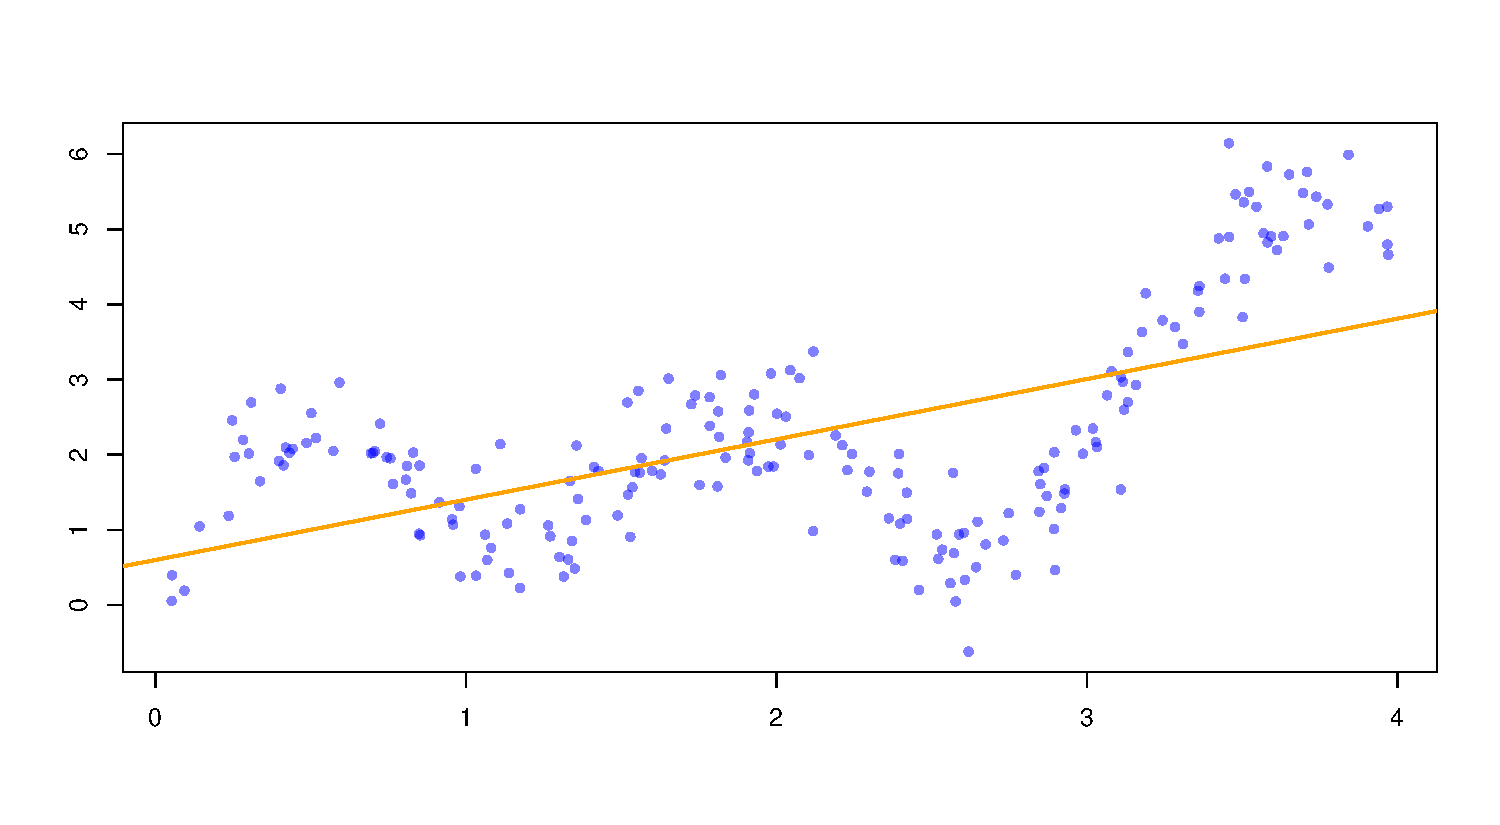
\includegraphics[width=\textwidth]{img/olsSimple.pdf}
\end{center}

\end{frame}

%%%%%%%%%%%%%%%%%%%%%%%%%%%%%%%%%%%%%%%%%%%%%%%%%%%
\begin{frame}[fragile] \frametitle{} \oldB \small

\yblue{\textbf{Linear regression}}

Why might ordinary least squares be useful in non-parametric
regression? \pause \magenta{basis functions!}

\pause We can expand the model to include non-linear terms.
For example, we can expand to write $y$ as a power basis:
\begin{align*}
y_i &= \beta_0 + \sum_{j=1}^p x_i^j \cdot \beta_j + \epsilon_i
\end{align*}
Or as a Fourier basis:
\begin{align*}
y_i &= \beta_0 + \sum_{j=1}^p \sin(x_i * j) \cdot \beta_{2j} + \cos(x_i * j) \cdot \beta_{2j+1} + \epsilon_i
\end{align*}

\end{frame}

%%%%%%%%%%%%%%%%%%%%%%%%%%%%%%%%%%%%%%%%%%%%%%%%%%%
\begin{frame}[fragile] \frametitle{} \oldB \small

\yblue{\textbf{Linear regression}}

With enough terms this basis expansion can approximate nearly
all functional forms of $g$.

\end{frame}


%%%%%%%%%%%%%%%%%%%%%%%%%%%%%%%%%%%%%%%%%%%%%%%%%%%
\begin{frame}[fragile] \frametitle{} \oldB \small

\yblue{\textbf{local regression (LOESS)}}

Local regression combines the ideas of kernel smoothers and linear
regression. A separate linear regression is fit at each input point
$x_{new}$ for which $\widehat{g}$ is to be evaluated at. The regression
uses sample weights based on how for each sample is from $x_{new}$.

\pause One can use linear regression or use higher order polynomials.
Typically at most cubic functions are used.

\end{frame}

%%%%%%%%%%%%%%%%%%%%%%%%%%%%%%%%%%%%%%%%%%%%%%%%%%%
\begin{frame}[fragile] \frametitle{} \oldB \small

\begin{center}
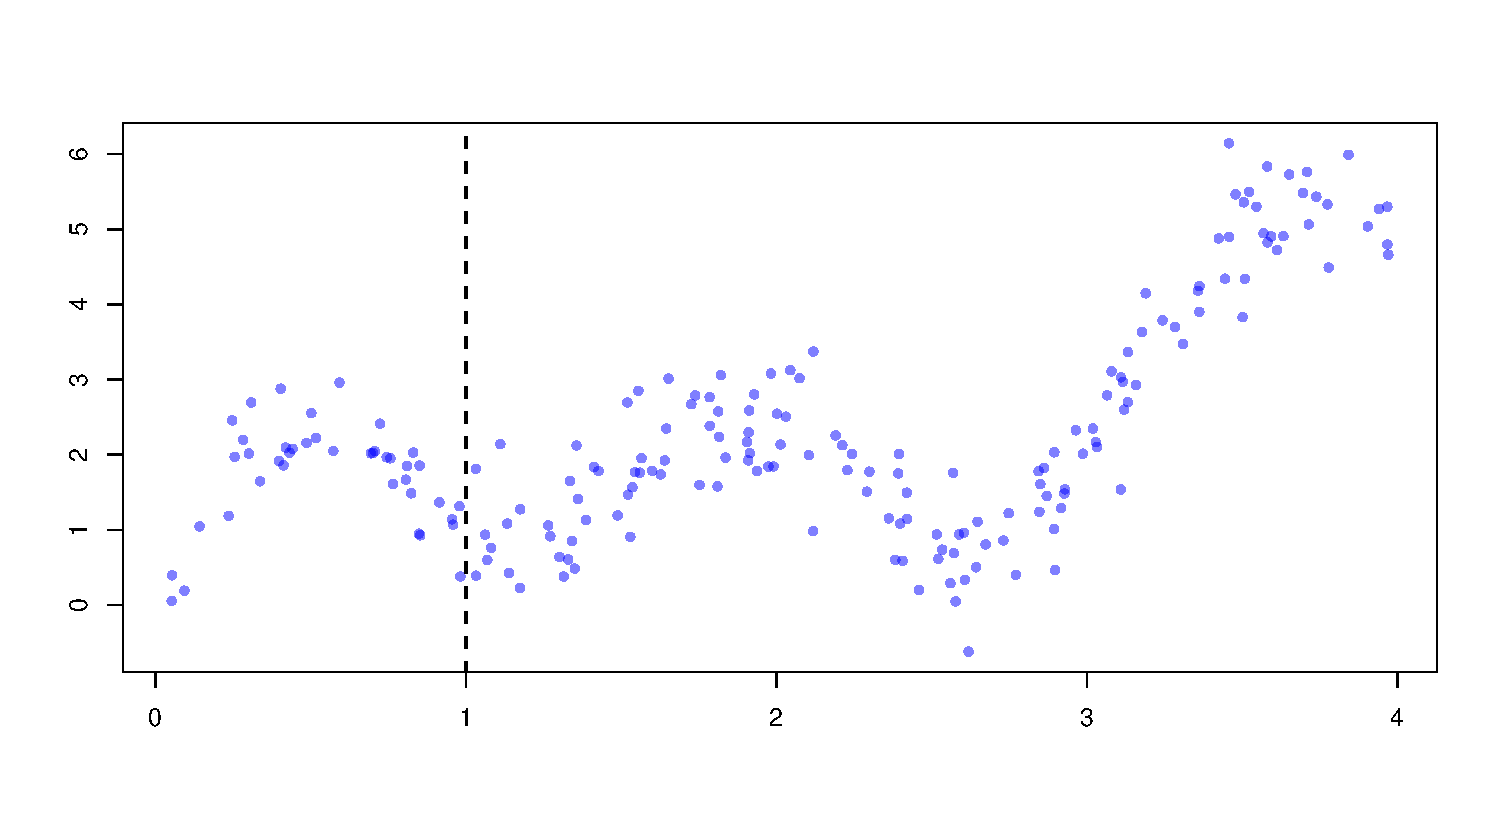
\includegraphics[width=\textwidth]{img/lowess1.pdf}
\end{center}

\end{frame}

%%%%%%%%%%%%%%%%%%%%%%%%%%%%%%%%%%%%%%%%%%%%%%%%%%%
\begin{frame}[fragile] \frametitle{} \oldB \small

\begin{center}
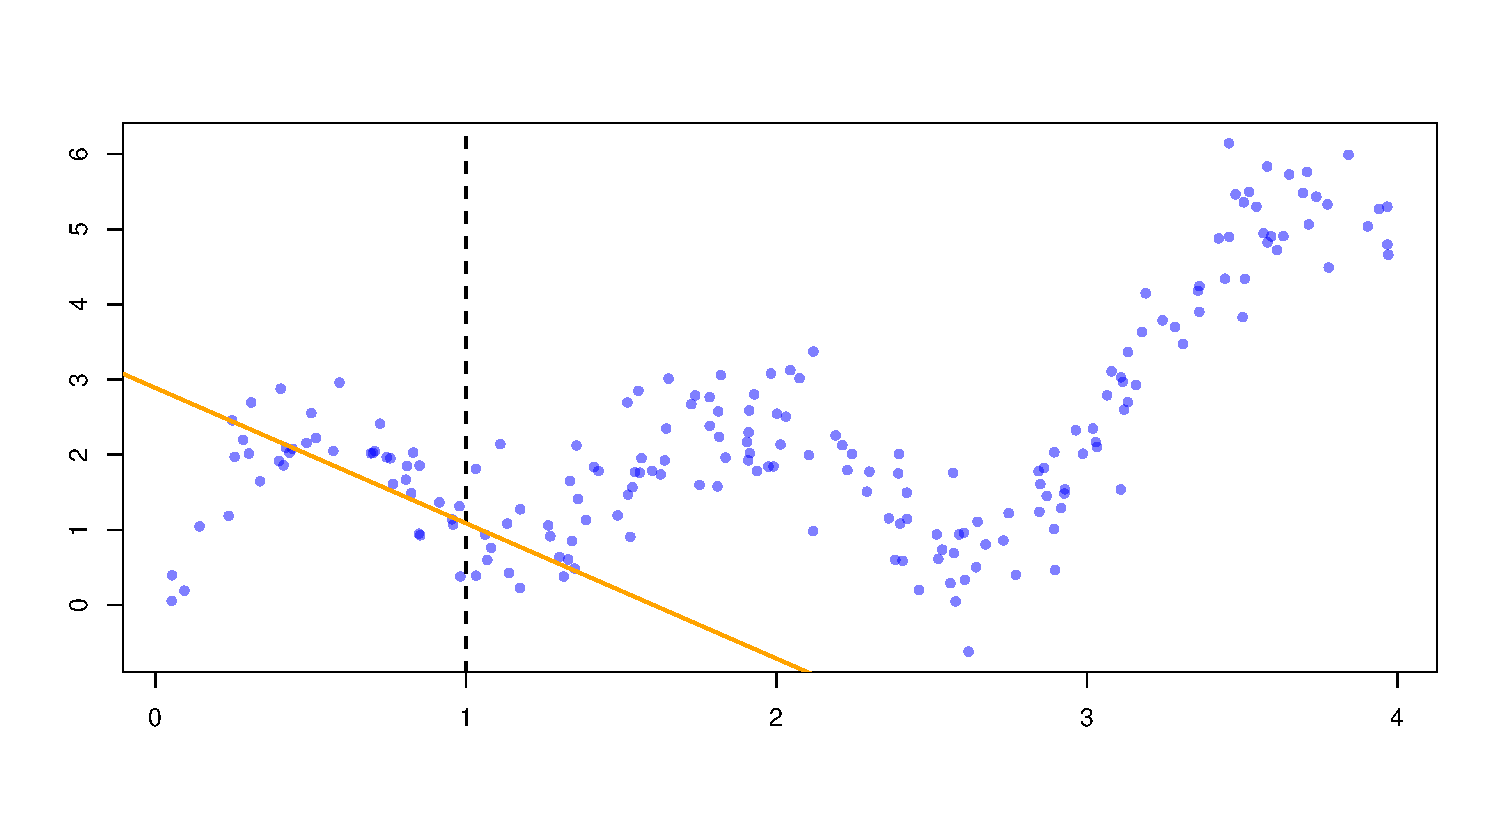
\includegraphics[width=\textwidth]{img/lowess2.pdf}
\end{center}

\end{frame}

%%%%%%%%%%%%%%%%%%%%%%%%%%%%%%%%%%%%%%%%%%%%%%%%%%%
\begin{frame}[fragile] \frametitle{} \oldB \small

\begin{center}
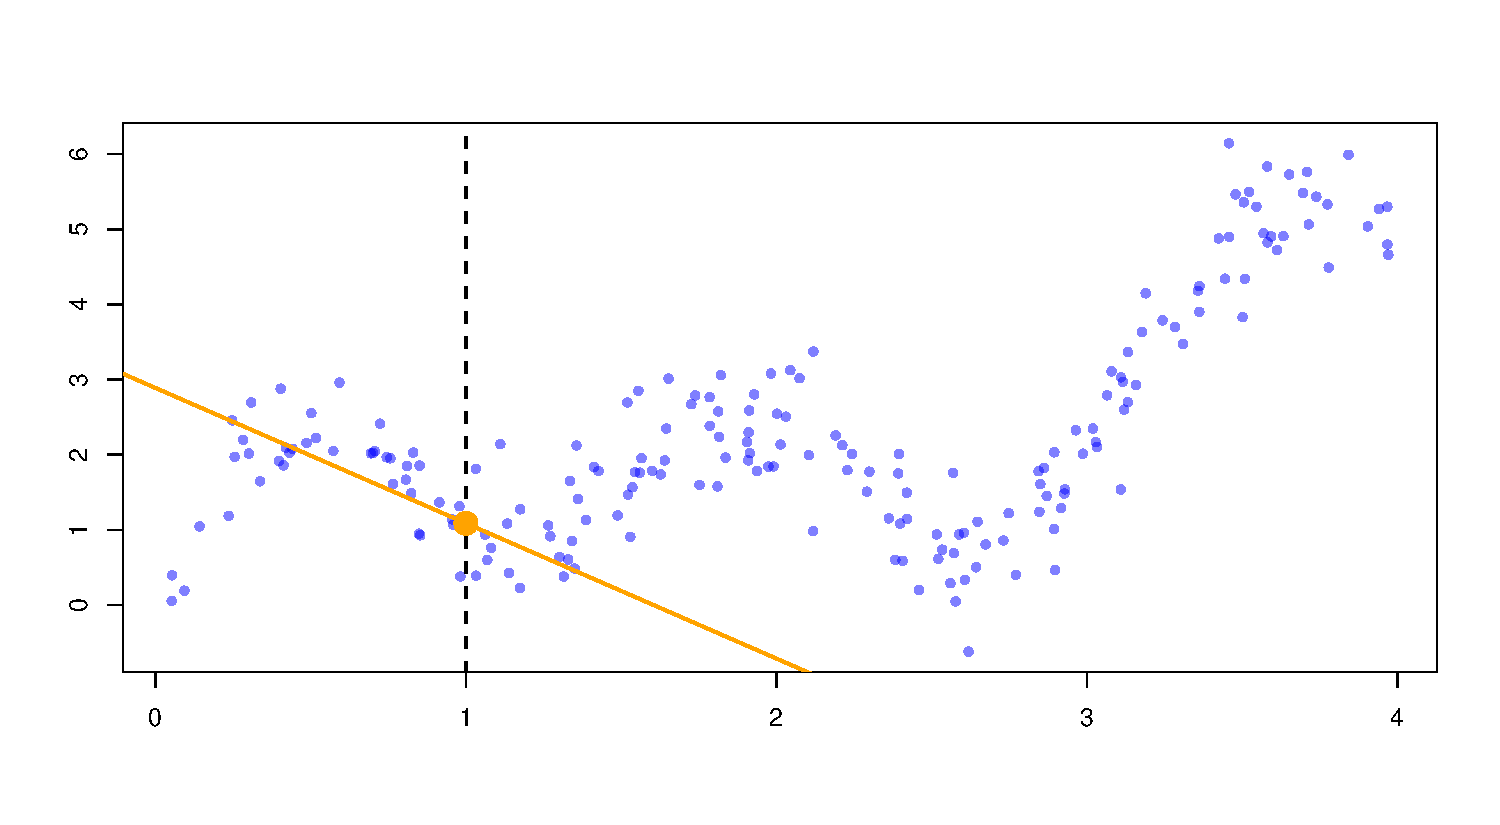
\includegraphics[width=\textwidth]{img/lowess3.pdf}
\end{center}

\end{frame}

%%%%%%%%%%%%%%%%%%%%%%%%%%%%%%%%%%%%%%%%%%%%%%%%%%%
\begin{frame}[fragile] \frametitle{} \oldB \small

\yblue{\textbf{Linear smoothers}}

How are these four techniques all related?\pause

All of them can be written as:
\begin{align*}
\widehat{y}_{new} &= \sum_i w_i y_i
\end{align*}
Where the weights $w_i$ depend only on the values $x_i$ (and $x_{new}$)
and not on the values of $y_i$.

\pause Anything that can be written in this form is called
a \blue{linear smoother}.

\end{frame}

%%%%%%%%%%%%%%%%%%%%%%%%%%%%%%%%%%%%%%%%%%%%%%%%%%%
\begin{frame}[fragile] \frametitle{} \oldB \small

\yblue{\textbf{Linear smoothers, cont.}}

For example, in the case of knn, the weights are $\frac{1}{k}$
for the $k$ closest values and $0$ for the remained of them.

\pause We have already seen the weights for the kernel smoother.

\pause The weights for ordinary least squares are given by our
derived ordinary least squares estimator:
\begin{align*}
w &= x_{new} (X^t X)^{-1} X^t
\end{align*}
And LOWESS is simply a sample weighted variant of this.

\end{frame}

%%%%%%%%%%%%%%%%%%%%%%%%%%%%%%%%%%%%%%%%%%%%%%%%%%%
\begin{frame}[fragile] \frametitle{} \oldB \small

\yblue{\textbf{Still to come\ldots}}

\begin{itemize}
\item computational issues of computing them
\item how to pick tuning parameters and choose amongst them
\item what happens when we have higher dimensional spaces
\end{itemize}

\end{frame}



\end{document}













